\section{Grundzüge der Integralrechnung}

Wir können die mathematische Operation des Integrierens auffassen als die Umkehrung der Differentiation. Das heißt: Wir suchen zu einer gegebenen Funktion $f(x)$ eine sogenannte \emph{Stammfunktion} $F(x)$, sodass 
\begin{align}
    f(x) = \dv{F(x)}{x} \qq{und schreiben} F(x) = \int f(x) \dd{x}.
\end{align}
Wir nennen dies das unbestimmte Integral der Funktion $f(x)$. In symbolischer schreibweise lässt sich das Integral folgendermaßen konstruieren: 
\begin{align}
    f(x) &= \dv{F(x)}{x} \quad |\cdot \dd{x} \notag \\
    f(x) \dd{x} &= \dv{F(x)}{x}\dd{x} = \dd{F}(x) \quad \bigg|\; \int \notag \\
    \int f(x) \dd{x} &= \int \dd{F(x)} = F(x).    
\end{align}
Ein paar Beispiele wollen wir hier beispielhaft einmal notieren. Kennen wir die Ableitungen verschiedener Funktionen, so können wir das dazugehörige Integral leicht konstruieren: 
\begin{multicols}{2}
    \begin{itemize}
        \item $\displaystyle \int 1 \dd{x} = x + C,$
        \item $\displaystyle \int x^n \dd{x} = \frac{x^{n+1}}{(n+1)} + C,$
        \item $\displaystyle \int \frac{1}{\sqrt{x}} \dd{x} = 2\sqrt{x} + C,$
        \item $\displaystyle \int \frac{1}{x} \dd{x} = \ln|x| + C,$
        \item $\displaystyle \int \frac{1}{1+x^2} \dd{x} = \arctan(x) + C,$
        \item $\displaystyle \int \e^{cx} \dd{x} = \frac{\e^{cx}}{c} + C.$
    \end{itemize}
\end{multicols}
Hierbei ist $C = \text{const.}$ die sogennante \emph{Integrationskonstante}. Das unbestimmte Integral beschreibt nämlich die Menge aller Stammfunktionen, deren erste Ableitung $f(x)$ ergibt. 

Im Gegensatz zur Differentiation existiert im Allgemeinen kein Algorithmus zur Bestimmung eines Integrals. Außerdem besitzt nicht jede Funktion eine geschlossen analytisch darstellbare Stammfunktion.

\paragraph{Beispiele}$~$\\[-2.2cm]

\begin{align}
    \text{Stammfunktion von} \quad f(x) &= 3xy^2 + 2y - 4x +3 \\
    F(x) &= \int (3xy^2 + 2y - 4x + 3) \dd{x} \notag \\
         &= \frac{3}{2} x^2 + y^2 + 2xy - 2x^2 + 3x + C \notag \\
         &= \qty(\frac{3y^2}{2} - 2)x^2 + (2y-3)x + C \notag \\
    \text{Stammfunktion von} \quad f(y) &= 3xy^2 + 2y - 4x +3 \\
    F(y) &= \int (3xy^2 + 2y - 4x + 3) \dd{y} \notag \\
         &=xy^3 + y^2 - (4x-3)y + C.\notag \\[-1.5cm] \notag 
\end{align}

Wir sehen also, dass es wichtig, ist, die korrekte Variable zur Integration auszuwählen. 

Bei einem \emph{bestimmten Integral} wird die Stammfunktion an einer oberen und einer unteren Grenze ausgewertet. Das Ergbnis hängt nicht mehr von der Integrationsvariablen ab. Wir können damit den \emph{Hauptsatz der Differential- und Integralrechnung} formulieren: 
\begin{mymathbox}[ams align, title={Hauptsatz der Integral- und Differentialrechnung}, colframe={FSUblau}]
    \int\limits_{x_1}^{x_2} f(x) \dd{x} = F(x_1) - F(x_1).
\end{mymathbox}
Man schreibt auch $\displaystyle \int\limits_{x_1}^{x_2} f(x) \dd{x} = F(x)\eval_{x_1}^{x_2}.$

Als Integrationsgrenze kann ebenfalls $\pm \infty$ auftauchen, was im Sinne eines Grenzwertes zu verstehen ist, also 
\begin{align}
    \int\limits_{0}^{\infty} f(x) \dd{x} = \lim_{t\to \infty} \int\limits_{0}^{t} f(x) \dd{x}.
\end{align}
Man findet außerdem oft Schreibweisen wie 
\begin{align}
    \int\limits_{-\infty}^{\infty} f(x) \dd{x} = \int\limits_{\mathbb{R}} f(x) \dd{x}.
\end{align}
Es ist zu beachten, dass sowohl endliche als auch unendliche Integrale nicht immer konvergent sind, bspw. 
\begin{align}
    \begin{split}
        \int\limits_{0}^{\infty} \e^{x} \dd{x} &= \e^{x}\eval_0^\infty \to \infty, \qquad \int\limits_{0}^{10} \frac{1}{r^2} \dd{x} = -\frac{1}{r}\eval_0^{10} \to \infty, \\
        \int\limits_{0}^{\infty} \cos(x) \dd{x} &= \sin(x)\eval_0^\infty \to \quad ? \;.
    \end{split}
\end{align}

\subsection{Das Wegintegral}

Wir führen das Wegintegral ein am Beispiel der Frage ``\emph{Was ist die Arbeit?}''. Bewegt sich ein Teilchen (Massepunkt) unter dem Einfluss einer konstanten Kraft $F$ entlang eines Weges der Länge $s$, dann lautet die Antwort 
\begin{align}
    \text{Arbeit } = \text{ Kraft mal Weg,} \qq{bzw.} W = F\cdot s.
\end{align}
Betrachten wir das konkrete Beispiel eines Elektrons (Ladung $q = -e$) im Kondensator mit elektrischer Feldstärke $\bm{E}$, das sich unter Einfluss einer Coulomb-Kraft $\bm{F} = q \cdot \bm{E}$ bewegt. 
\begin{figure}[htp]
    \centering
    \begin{tikzpicture}
        \draw[thick] (-4,0) -- (-3,0);
        \draw[thick] (4,0) -- (3,0);
        \draw[thick] (-3,-1) -- (-3,1);
        \draw[thick] (3,-1) -- (3,1);
        \fill (-1,0) circle (2pt);
        \draw[very thick, -{latex}] (-1,0) --node[above]{$\bm{F}= q \cdot \bm{E}$} (1,0);
        \foreach \x in {0.8,0.6,...,-.8}{
            \draw[FSUblau, opacity=0.2, -{latex}] (3,\x) -- (-3,\x);
        }
        \draw[thick, {latex}-{latex}] ( -3,-1.2) --node[below]{s} (3,-1.2);
    \end{tikzpicture}
\end{figure}

Würden wir das elektrische Feld immer dann neu einstellen, wenn das Elektron ein bestimmtes Wegintervall $\Delta s$ zurückgelegt hat, so ergäbe sich die gesamte Arbeit als Summe der Arbeiten innerhalb der einzelnen Teilstrecken.
\begin{figure}[htp]
    \centering
    \begin{tikzpicture}
        \draw[thick] (-4,0) -- (-3,0);
        \draw[thick] (4,0) -- (3,0);
        \draw[thick] (-3,-1) -- (-3,1);
        \draw[thick] (3,-1) -- (3,1);
        % \fill (-1,0) circle (2pt);
        % \draw[very thick, -{latex}] (-1,0) --node[above]{$\bm{F}= -e \cdot \bm{E}$} (1,0);
        \foreach \x in {0.8,0.6,...,-.8}{
            \draw[FSUblau, opacity=0.2, -{latex}] (3,\x) -- (-3,\x);
        }
        \foreach \x in {-3,-2,-1,0,2}{
            \draw[thick, {latex}-{latex}] (\x,0.8) --node[above]{$\Delta s$} +(1,0);
        }
        \foreach \x in {-3,-2,-1,0,1}{
            \draw[dashed] (\x+1, 1) -- +(0,-2);
        }
        \node (A) at (-3+0.5,-0.5){$F_1$};
        \node (A) at (-2+0.5,-0.5){$F_2$};
        \node (A) at (-1+0.5,-0.5){$F_3$};
        \node (A) at (0+0.5,-0.5){$F_4$};
        \node (A) at (1+0.5,-0.5){$\hdots$};
        \node (A) at (2+0.5,-0.5){$F_n$};
        \draw[thick, {latex}-] ( -3,-0.8) --node[below]{s} (1.3,-0.8);
        \draw[thick, -{latex}] ( 1.7,-0.8) -- (3,-0.8);
        \node[anchor=west] (A) at (4.5,.3){$n$ Teilstücke};
        \node[anchor=west] (A) at (4.5,-.3){$s = n \cdot \Delta s$};
        \node (A) at (-6.5,0){};
    \end{tikzpicture}
\end{figure}
Für $n$ Teilstücke ergibt sich die Gesamt-Arbeit zu 
\begin{align}
    W &= W_1 + W_2 + \hdots + W_n \notag \\
      &= q E_1 \Delta s + q E_1 \Delta s + \hdots + e E_n \Delta s = q \sum_{i=1}^{s/\Delta s} E_i \Delta s.
\end{align}
Wollen wir nun die Gesamtarbeit bestimmen für den Fall, dass das $E$-Feld \emph{kontinuierlich} verändert wird, so habne wir den Weg in unendlich viele Intervalle einzuteilen, sodass das Feld in diesen unendlich kleinen (infinitesimalen) Intervallen konstant ist; das führt auf die Definition des Integrals: 
\begin{align}
    W = q \cdot \lim_{\Delta s \to 0} \qty(\sum_{i=1}^{s/\Delta s} E_i \Delta s) =: q\int\limits_{0}^{s} E(s') \dd{s'}.
\end{align}
Dabei ist das elektrische Feld nun als eine (kontinuierliche) Funktion $E = E(s)$ aufzufassen. Bildlich gesprochen heißt das: Mit Hilfe des Integrals ``bewegen'' wir uns entlang eines Weges und ``sammeln'' an allen Punkten die Beiträge der Kraft zur Gesamtarbeit ein. 
\begin{quote}
    Arbeit ist das Integral über eine Kraft entlang eines Weges.
\end{quote}
Der Weg muss hierbei nicht notwendigerweise gerade sein. 
\begin{figure}[htp]
    \centering
    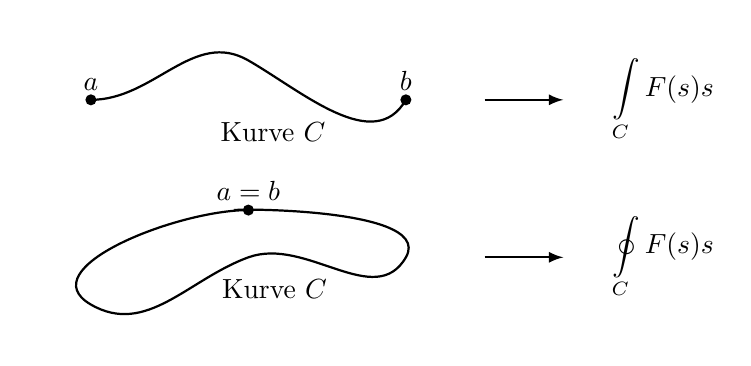
\begin{tikzpicture}
        \fill (0,0) circle (2pt)node[above]{$a$};
        \fill (4,0) circle (2pt)node[above]{$b$};
        \draw[thick] (0,0) to[out=0,in=150] (2,0.5) to [out=150-180, in =240]node[below left]{Kurve $C$} (4,0);
        \draw[thick, -{latex}] (5,0) -- (6,0);
        \node[anchor=west] at (6.5,0){$\displaystyle\int\limits_C \bm{F}(\bm{s}) \dd{\bm{s}}$};
        \begin{scope}[shift={(0,-2)}]
            \fill (2,0.6) circle (2pt)node[above]{$a=b$};
            \draw[thick] (2,0.6) to[out=180,in=150] (0,-.6) to [out=150-180, in =200](2,0) to [out=200-180, in=240]node[below left]{Kurve $C$}  (4,0) to [out=240-180, in=180] (2,0.6);
            \draw[thick, -{latex}] (5,0) -- (6,0);
            \node[anchor=west] at (6.5,0){$\displaystyle\oint\limits_C \bm{F}(\bm{s}) \dd{\bm{s}}$};
        \end{scope}
    \end{tikzpicture}
\end{figure}
Insbesondere können wir die Länge einer Kurve bestimmen als das Integral über die konstante Funktion $f(s) = 1$. Bildlich heißt das: Wir ``sammeln'' den Beitrag eines jeden infinitesimalen Streckenabschnitts zur Gesamtlänge ein.

\subsection{Flächen- und Volumenintegrale}

So wie wir Längen mit Hilfe des Wegintegrales berechnen können, lassen sich Flächen mit Hilfe von Flächenintegralen berechnen, 
\begin{align}
    \text{Doppelintegral: } \quad A = \iint\limits_{\text{Fläche}} \dd{x}\dd{y}. 
\end{align}

\paragraph{Beispiel: Das rechtwinklige Dreieck}$~$

\begin{wrapfigure}{r}{6cm}
    \centering
    \vspace{-5mm}
    \begin{tikzpicture}
        \draw[thick, -{latex}] (0,0) -- (4,0)node[right]{$x$};
        \draw[thick, -{latex}] (0,0) -- (0,2.5)node[above]{$y$};
        \draw [decorate, decoration = {calligraphic brace}, thick] (3.5,-.2) --node[below]{$a$}  (0,-.2);
        \draw [decorate, decoration = {calligraphic brace}, thick] (3.7,2) --node[right]{$b$}  (3.7,0);
        \draw[thick, {latex}-{latex}] (2.5,0) --node[right]{$x \frac{b}{a}$} (2.5, 2.5*2/3.5);
        \filldraw[draw=black, fill=FSUblau, fill opacity=0.4, thick] (0,0) -- (3.5,0) -- (3.5,2) -- cycle;
    \end{tikzpicture}
    \vspace{-2.4cm}
\end{wrapfigure}

Wir legen zunächst die Integrationsgrenzen fest: 
\begin{align}
    x \qq{von} &0 \qq{bis} a, \notag\\
    y \qq{von} &0 \qq{bis} \frac{b}{a}x \notag \\
    \Rightarrow A &= \int\limits_{0}^{a}\dd{x} \int\limits_{0}^{\frac{b}{a}x} \dd{y} = \int\limits_{0}^{a}\dd{x} y \eval_0^{\frac{b}{a}x} = \int\limits_{0}^{a} \frac{b}{a}x \dd{x} \notag \\
    &= \frac{b}{a} \int\limits_{0}^{a}x \dd{x} = \frac{b}{2a} x^2 \eval_0^a = \uuline{\frac{ab}{2}}.
\end{align}
In der Schule wird das Integral über eine Funktion $f(x)$ oft eingeführt als die Fläche, die diese Funktion mit der $x$-Achse einschließt:
\begin{align}
    A = \int\limits_{0}^{x_0} \dd{x} \int\limits_{0}^{f(x)} \dd{y} = \int\limits_{0}^{x_0} \dd{x} y \eval_0^{f(x)} = \int\limits_{0}^{x_0} f(x) \dd{x}.
\end{align}
Beachte, dass auch unendliche Flächenintegrale konvergieren können, wie bspw. 
\begin{align}
    A = \int\limits_{1}^{\infty} \frac{1}{r^2} \dd{r} = -\frac{1}{r}\eval_1^\infty = 1.
\end{align}
Es wird an dieser Stelle kaum verwunderlich sein, dass auch Volumen durch Integration bestimmt werden. Wir führen dafür das \emph{Volumenintegral} bzw. \emph{Dreifachintegral} ein 
\begin{align}
    V = \iiint\limits_{\text{Volumen}} \dd{x} \dd{y}\dd{z}.
\end{align}

\newpage
\paragraph{Beispiel: Prisma mit Parabelausschnitt}$~$

\begin{wrapfigure}{r}{6cm}
    \centering
    \vspace{-5mm}
    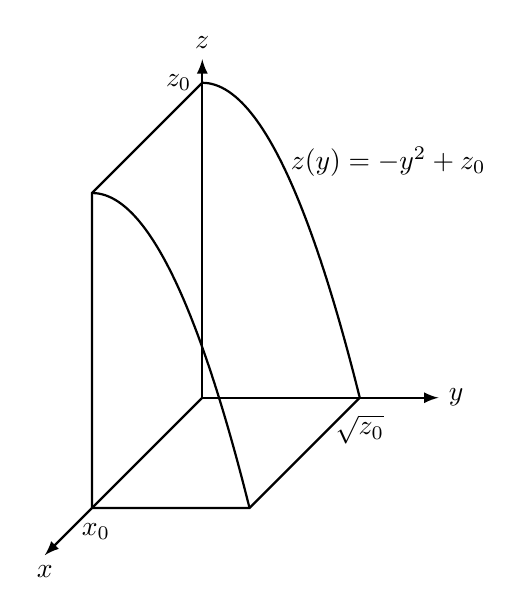
\begin{tikzpicture}
        \draw[thick, -{latex}] (0,0) -- (-2,-2)node[below]{$x$};
        \draw[thick, -{latex}] (0,0) -- (3,0)node[right]{$y$};
        \draw[thick, -{latex}] (0,0) -- (0,4.3)node[above]{$z$}; 
        \draw[ domain=0:2, smooth, variable=\x, thick] plot ({\x}, {-1*(\x)*(\x)+4});
        \draw[ domain=-1.4:0.6, smooth, variable=\x, thick] plot ({\x}, {-1*(\x+1.4)*(\x+1.4)+4-1.4});
        \draw[thick] (0,4) -- ++(-1.4,-1.4) -- ++(0,-4) -- ++(2,0) -- ++(1.4,1.4);
        \node (A) at (-1.35,-1.7){$x_0$};
        \node (A) at (2,-.4){$\sqrt{z_0}$};
        \node[anchor=west] (A) at (1,3){$z(y) = -y^2 +z_0$};
        \node (A) at (-.3,4){$z_0$};
    \end{tikzpicture}
    \vspace{-6cm}
\end{wrapfigure}

Das Volumen des Prismas ergibt sich zu 
\begin{align}
    V &= \int\limits_{0}^{x_0} \dd{x} \int\limits_{0}^{\sqrt{z_0}} \dd{y} \int\limits_{0}^{-y^2 + z_0} \dd{z} \notag \\
    &= \int\limits_{0}^{x_0} \dd{x} \int\limits_{0}^{\sqrt{z_0}} \dd{y} ( -y^2 + z_0) \notag \\
    &= \int\limits_{0}^{x_0} \dd{x} \eval(-\frac{y^3}{3}+z_0 y|_0^{\sqrt{z_0}} \notag \\
    &= x_0 \qty(-\frac{\sqrt{z_0}^3}{3} + z_0 \sqrt{z_0}) = \uuline{\frac{2}{3} x_0 \sqrt{z_0}^3}.
\end{align}
Hierbei ``laufen'' die Integrale über $x$ und $y$ die Grundfläche ab, während das $z$-Integral mit der (von $y$ abhängigen) Höhe multipliziert wird. 

\emph{Bemerkung: } Man schreibt auch $A = \iint \dd{x}\dd{y} = \int \dd{A}$ und $V = \iiint \dd{x}\dd{y}\dd{z} = \int \dd{V}$, sodass eine bildliche Vorstellung ähnlich dem Wegintegral möglich ist: Wir schreiten das Gebiet innerhalb der Integrationsgrenzen ab und ``sammeln'' infinitesimale Flächenstücke $\dd{A}$ bzw. Volumenstücke $\dd{V}$ ein.

Natürlich können auch Flächen- und Volumenintegrale über Funktionen betrachtet werden. Dafür betrachten wir beispielhaft die Masse eines Quaders der Kantenlängen $a,b,c$, dessen Dichte $\varrho$ ortsabhängig ist: 
\begin{align}
    M = \int\limits_{0}^{a}\dd{x} \int\limits_{0}^{b}\dd{y} \int\limits_{0}^{c}\dd{z} \varrho(x,y,z) = \int\limits_{V} \varrho(\bm{r}) \dd{V}.
\end{align}

\subsection{Eigenschaften und Rechenregeln}

\begin{itemize}
    \item Linearität: $\displaystyle \int\limits_{a}^{b} \qty(\alpha f(x)+\beta g(x)) \dd{x} = \alpha \int\limits_{a}^{b} f(x) \dd{x} + \beta \int\limits_{a}^{b} g(x) \dd{x}$ 
    \item Zerlegung des Integrationsgebietes: $a < k < b$ 
    \begin{align}
        \int\limits_{a}^{b} f(x) \dd{x} = \int\limits_{a}^{k} f(x) \dd{x} + \int\limits_{k}^{b} f(x) \dd{x}
    \end{align}
    \item Vertauschung der Grenzen: $\displaystyle \int\limits_{a}^{b} f(x) \dd{x} = - \int\limits_{b}^{a}f(x) \dd{x}$\\
    Speziell für \emph{gerade Funktionen}, $f(-x) = f(x)$ bzw. \emph{ungerade Funktionen}, $f(-x) = -f(x):$
    \begin{align}
        \int\limits_{-a}^{a} f(x) \dd{x} &= \underbrace{\int\limits_{-a}^{0}f(x) \dd{x}} + \int\limits_{0}^{a} f(x) \dd{x} = \begin{cases}
            2 \int\limits_{0}^{a} f(x) \dd{x} & f(-x) = f(x)\\ 0 & f(-x) = -f(x)
        \end{cases} \\
        & \qquad = -\int\limits_{0}^{-a} f(x) \dd{x} = \int\limits_{0}^{a} f(-x) \dd{x}, \quad \text{nach Subst. } x \to -x, \quad \dd{x} \to -\dd{x} \notag 
    \end{align}
    Beispiel 1: $f(x) = \cos (x)$ 
    \begin{align}
        \int\limits_{-\pi/2}^{\pi/2} \cos(x) \dd{x} = \sin(x)\eval_{-\frac{\pi}{2}}^{\frac{\pi}{2}}= 2,   \qquad 2 \int\limits_{0}^{\pi/2} \cos(x)\dd{x} = 2 \sin(x)\eval_0^{\frac{\pi}{2}} = 2.
    \end{align}
    % Speziell für \emph{ungerade Funktionen}, $f(-x) = -f(x):$
    % \begin{align}
    %     \int\limits_{-a}^{a} f(x) \dd{x} &= \underbrace{\int\limits_{-a}^{0}f(x) \dd{x}} + \int\limits_{0}^{a} f(x) \dd{x} = 0\\
    %     & \qquad = -\int\limits_{0}^{-a} f(x) \dd{x} = \int\limits_{0}^{a} f(-x) \dd{x}, \quad \text{nach Subst. } x \to -x, \quad \dd{x} \to -\dd{x} \notag 
    % \end{align}
    Beispiel 2: $f(x) = \sin (x)$ \vspace{-4mm}
    \begin{align}
        \int\limits_{-\pi}^{\pi} \sin(x) \dd{x} = -\cos(x)\eval_{-\pi}^{\pi} = 1+(-1) = 0.
    \end{align}
    \item Umkehrung der Ableitung: $\int \dv{f}{x} \dd{x} = \int \dd{f} = f.$
\end{itemize}

\paragraph{Beispiel: Bewegung mit konstanter Beschleunigung}$~$

Wir gehen nun von einer konstant beschleunigten (Beschleunigung $a$) Bewegung ($v(t)$ - Geschwindigkeit) aus: 
\begin{align}
    \dv{v(t)}{t} &= a \quad \bigg| \int \dd{t'} \\ 
    \int\limits_{t_0}^{t} \dv{v(t')}{t'} \dd{t'} &= \int\limits_{t_0}^{t} a \dd{t'} \quad \Rightarrow \quad\int\limits_{v(t_0)}^{v(t)} \dd{v} = a \cdot (t-t_0) \notag \\
    v(t) - v(t_0) &= a\cdot (t-t_0)\qq{, wähle $t_0=0$ und $v(0) \equiv v_0$} \notag \\
    \Rightarrow v(t) &= a\cdot t + v_0. 
\end{align}
Nun berechnen wir noch die Funktion des Ortes $x(t)$ durch eine zweite Integration
\begin{align}
    \dv{x(t)}{t} &= v(t) = a\cdot t + v_0 \quad \bigg| \int \dd{t'} \\ 
    \int\limits_{0}^{t} \dv{x(t')}{t'} \dd{t'} &= \int\limits_{0}^{t} (a\cdot t' + v_0) \dd{t'} \quad \Rightarrow \quad\int\limits_{x(0)}^{x(t)} \dd{x} = a \cdot \frac{t^2}{2} + v_0 t \notag \\
    x(t) - x(0) &= \frac{a}{2} t^2 + v_0 t\qq{, $x(0) \equiv x_0$} \notag \\
    \Rightarrow x(t) &= \uuline{\frac{a}{2}t^2 + v_0 t + x_0}. 
\end{align}

Im Folgenden werden noch drei besonders wichtige Methoden zur Umformung von Integralen vorgestellt. 

\paragraph{1. Partielle Integration}$~$

Hier sind: $u=u(x), v=v(x)$ Funktionen und $u' = \dv{u(x)}{x}, v' = \dv{v(x)}{x}$. 

Wir wenden nun die Produktregel der Differentiation auf das Produkt $u\cdot v$ an und integrieren anschließend wieder: 
\begin{align}
    (u v)' = u' v + v' u  \qq{bzw.} u v' = (u v)' - vu'  \quad \bigg| \int \dd{x}
\end{align}
\begin{mymathbox}[ams align, title={Partielle Integration}, colframe={FSUblau}]
    \int u(x) v'(x) \dd{x} &= u(x) v(x) - \int v(x) u'(x) \dd{x} \\
    \qq{mit Grenzen} \int\limits_{a}^{b} u(x) v'(x) \dd{x} &= u(x) v(x)\eval_a^b - \int\limits_a^b v(x) u'(x) \dd{x}
\end{mymathbox}

\begin{alignat}{3}
    &\qq{Beispiel 1:}& \int \underbrace{x}_{u} \underbrace{\e^{x}}_{v'} \dd{x}  &= x \e^x - \int \e^x \dd{x} = \uuline{(x-1) \e^x + C}.\\
    &\qq{Beispiel 2:}& \int \ln(x) \dd{x} &= x \ln(x) - \int \dd{x} = \uuline{x(\ln x -1) + C}. \\
    & &&\quad\begin{rcases}
        u = \ln(x) \\ v' = 1 
    \end{rcases} u' = \frac{1}{x}, \quad v= x \notag \\
    &\qq{Beispiel 3:}& \int \sin(x)\cos(x) \dd{x} &= -\cos^2(x) - \int \sin(x) \cos(x) \dd{x}. \notag \\
    & &&\quad \begin{rcases}
        u = \cos(x) \\ v' = \sin(x) 
    \end{rcases} u' = -\sin(x), \quad v= -\cos(x) \notag \\
    & &\hspace{-1cm}\Rightarrow 2 \int \sin(x) \cos(x) \dd{x} &= -\cos^2(x) + C \notag \\
    & &            \int \sin(x) \cos(x) \dd{x} &= \uuline{-\frac{1}{2}\cos^2(x) + \tilde{C}}
\end{alignat}
Bemerkung: Für das letzte Beispiel, kann das Integral mithilfe des Additionstheorems~\eqref{eqn:07_Doppelwinkel_sin} vereinfacht werden zu $\frac{1}{2}\sin(2x)$, wodurch sich das Integral einfach berechnen lässt zu 
\begin{align}
    \frac{1}{2}\int \sin(2x) \dd{x} = -\frac{1}{4} \underbrace{\cos(2x)}_{\mathclap{2 \cos^2(x) -1}} + C  = -\frac{1}{2} \cos^2(x) + \underbrace{\frac{1}{4} + C}_{\tilde{C}}.
\end{align}
Hier erkennen wir, wie wichtig die Integrationskonstante beim Integrieren ist. Durch das Additionstheorem ist die erhaltene Stammfunktion um $\frac{1}{4}$ gegenüber der vorherigen Methode nach unten verschoben gewesen.

\paragraph{2. Logarithmische Integration}$~$

Steht bei der Integration eines Bruches die Ableitung des Nennerterms im Zähler, so lässt sich das zugehörige Integral einfach berechnen: 
\begin{mymathbox}[ams align, title={Logarithmische Integration}, colframe={FSUblau}]
    \int \frac{f'(x)}{f(x)} \dd{x} = \ln|f(x)| + C.
\end{mymathbox}

\begin{alignat}{3}
    &\qq{Beispiel 1:}& \int \frac{3x^2+10x+2}{x^3+5x^2+2x} \dd{x} &= \uuline{\ln|x^3+5x^2+2x| + C}. \\
    &\qq{Beispiel 2:}& \int \frac{1}{\cos^2(x)\tan(x)} \dd{x} &= \int \frac{\frac{1}{\cos^2(x)}}{\tan(x)} \dd{x} = \uuline{\ln|\tan(x)| + C}.
\end{alignat}

\paragraph{3. Substitution}$~$

Durch Substitution erfolgt ein Wechsel der Integrationsvariable: 
\begin{align}
    \int\limits_{a}^{b} f(x) \dd{x} &\qq{, betrachte $z=z(x)$ bzw. $x(z)$} \notag \\
    & \Rightarrow \qq{Wechsel der Grenzen} a \mapsto z(a), \quad b \mapsto z(b) \notag \\
    & \Rightarrow \qq{Wechsel des Integrationsmaßes:} \dv{x(z)}{z} = x' \rightarrow \dd{x} = x'(z) \dd{z} \notag \\
    \int\limits_{a}^{b} f(x) \dd{x} &= \int\limits_{z(a)}^{z(b)} f(x(z)) x'(z) \dd{z}. 
\end{align}

\begin{alignat}{3}
    &\qq{Beispiel 1:}& \int \tan(x) \dd{x} &, \qq{Substitution:} z(x) = \tan(x)\\
    & & \dv{z}{x} &= 1 + \tan^2(x) = 1+z^2 \quad \Rightarrow \quad \dd{x} = \frac{\dd{z}}{1+z^2} \notag \\
    & & \Rightarrow \int \tan(x) \dd{x} &= \int \frac{z}{1+z^2} \dd{z} = \frac{1}{2} \ln(1+z^2) + C = \frac{1}{2} \underbrace{\ln(1+\tan^2(x))}_{\mathclap{1+\tan^2(x) = \cos^{-2}(x)}} + C \notag \\
    & & &= \frac{- \ln(\cos^2(x))}{2} + C = \uuline{-\ln|\cos(x)| + C}.
\end{alignat}

\begin{alignat}{3}
    &\qq{Beispiel 2:}& \int\limits_0^{\pi/2} \sin^3(x)\cos(x) \dd{x} &, \qq{Substitution:} z(x) = \sin(x), \quad \dv{z}{x} = \cos(x) \notag \\
    & & \text{Grenzen: } x&=0: z=0, \quad x = \frac{\pi}{2}: z=1, \qq{Maß:} \dd{x} = \frac{\dd{z}}{\cos(x)} \notag \\
    & & \Rightarrow \int\limits_0^{\pi/2} \sin^3(x)\cos(x) \dd{x} &= \int\limits_{0}^{1} z^3 \dd{z} = \frac{z^4}{4}\eval_0^1 = \uuline{\frac{1}{4}}. 
\end{alignat}

\paragraph{Integrationstabelle}$~$

Im Folgenden wollen wir noch einmal einige häufige Integrale zusammenstellen.
\begin{table}[htp]
    \centering
    \caption{Integrale spezieller Funktionen}
    \begin{tabular}[t]{l l}
        \toprule
        $f(x)$ & $F(x) + C$ \\
        \midrule 
        $x^n$ & $\dfrac{1}{n+1} x^{n+1}$ \\
        $\dfrac{1}{x}$ & $\ln|x|$ \\[2mm]
        $\e^x$ & $\e^x$ \\
        $a^x$ & $\dfrac{a^x}{\ln a}$ \\[2mm]
        $\sin(x)$ & $-\cos(x)$ \\
        $\cos(x)$ & $\sin(x)$ \\
        $\dfrac{1}{\cos^2(x)}$ & $\tan(x)$ \\
        $\dfrac{1}{\sin^2(x)}$ & $-\cot(x)$ \\
        $\dfrac{1}{\sqrt{1-x^2}}$ & $\arcsin(x)$ \\
        $\dfrac{1}{1+x^2}$ & $\arctan(x)$ \\
    \end{tabular}
    \hspace{1cm}
    \begin{tabular}[t]{l l}
        \toprule
        $f(x)$ & $F(x) + C$ \\
        \midrule 
        $\ln x$ & $x(\ln x- 1)$ \\[2mm]
        $\log_a x$ & $\dfrac{x}{\ln a}(\ln x- 1)$ \\[2mm]
        $\tan x$ & $-\ln|\cos x|$ \\[2mm]
        $\cot x$ & $\ln|\sin x|$ \\[2mm] 
        $\arcsin x$ & $x \arcsin x + \sqrt{1-x^2}$ \\[2mm]
        $\arccos x$ & $x \arccos x - \sqrt{1-x^2}$ \\[2mm]
        $\arctan x$ & $x \arctan x - \dfrac{1}{2} \ln(1+x^2)$\\[2mm]
        $\text{arccot} \,x$ & $x \,\text{arccot}\, x + \dfrac{1}{2} \ln(1+x^2)$
    \end{tabular}
\end{table}